\documentclass[11pt,letterpaper]{article}

% ----------------------------------------------------------------------
%  Paquetes
% ----------------------------------------------------------------------
\usepackage[utf8]{inputenc}
\usepackage[T1]{fontenc}
\usepackage[spanish,es-nodecimaldot,es-tabla]{babel}
\providecommand{\spanishplainpercent}{}\spanishplainpercent   % el signo % sin espacio automatico
\usepackage{lmodern}
\usepackage[margin=2.2cm]{geometry}
\usepackage{amsmath,amssymb}
\usepackage{graphicx}
\usepackage{booktabs}
\usepackage{array}
\usepackage{float}
\usepackage{caption}
\usepackage{xcolor}
\usepackage{listings}
\usepackage{tikz}
\usetikzlibrary{babel,arrows.meta,calc}   % babel: evita conflicto de babel-spanish con TikZ
\usepackage{hyperref}

\graphicspath{{IMAGENES/}}
\captionsetup{font=small,labelfont=bf}
\hypersetup{colorlinks=true,linkcolor=blue!50!black,urlcolor=blue!50!black,citecolor=blue!50!black}

\lstset{
  language=Matlab,
  basicstyle=\ttfamily\footnotesize,
  keywordstyle=\color{blue!70!black}\bfseries,
  commentstyle=\color{green!45!black},
  stringstyle=\color{purple!80!black},
  frame=single, framerule=0.3pt, rulecolor=\color{gray!60},
  backgroundcolor=\color{gray!6},
  breaklines=true, columns=fullflexible,
  showstringspaces=false,
  literate={á}{{\'a}}1 {é}{{\'e}}1 {í}{{\'i}}1 {ó}{{\'o}}1 {ú}{{\'u}}1 {ñ}{{\~n}}1
}

\newcommand{\R}{\mathbb{R}}

% ----------------------------------------------------------------------
\title{\textbf{Diseño e implementación en simulación de un controlador MIMO\\
en espacio de estados para un carro eléctrico\\ de tracción trasera con dos motores}\\[4pt]
\large Punto 3 -- Proyecto de tercera nota, Sistemas de Control II}
\author{Santiago Alexander Bravo Rodriguez -- 2224734\\
Escuela de Ingenierías Eléctrica, Electrónica y de Telecomunicaciones\\
Universidad Industrial de Santander}
\date{Noviembre de 2026}

\begin{document}
\maketitle

\begin{abstract}
Se diseña e implementa en simulación un controlador de múltiples entradas y múltiples salidas (MIMO) en espacio de estados para un carro eléctrico pequeño de tracción trasera. El carro tiene dos motores DC JGB37-555B independientes, uno por rueda trasera, cuyo modelo se obtuvo en el punto~2. Las entradas son los voltajes de los motores izquierdo y derecho, y las salidas son la velocidad de avance $v$ y la velocidad de giro $\Omega$. Como ambos motores empujan la misma masa, cada voltaje afecta a las dos salidas: el sistema es acoplado. A partir de las leyes de Newton y de Kirchhoff se obtiene un modelo de cuatro estados que se reduce a dos estados para el diseño. Se diseña un regulador cuadrático lineal discreto (LQR) con acción integral sobre $v$ y $\Omega$, con una sola matriz de ganancias de $2\times4$, y un filtro de Kalman discreto que combina los encoders de las ruedas con un giroscopio y estima las perturbaciones. El controlador se implementa en MATLAB sobre una planta no lineal con corrientes de motor, motores desiguales, fricción de Coulomb, saturación de $\pm12$~V, encoders cuantizados, ruido en el giroscopio, una pendiente y un freno en una rueda. Se compara con dos controladores PI independientes, uno por rueda. El LQR MIMO cumple todas las especificaciones, reduce el giro indeseado durante un arranque recto de 0.126 a 0.035~rad/s y el error de rumbo al final del recorrido de 0.136 a 0.014~rad.
\end{abstract}

\tableofcontents
\bigskip

% ======================================================================
\section{Introducción}
% ======================================================================
El punto~3 del proyecto pide diseñar e implementar un controlador MIMO en espacio de estados sobre el sistema elegido. El sistema es un carro eléctrico pequeño con \textbf{dos motores independientes en el eje trasero}, sin dirección mecánica: el carro gira cuando las dos ruedas traseras giran a velocidades distintas. En los vehículos eléctricos esta técnica se conoce como \emph{diferencial electrónico} o \emph{torque vectoring}.

Cada motor es un JGB37-555B, cuyo modelo y controlador de posición se desarrollaron en el punto~2. Aquí se reutilizan los mismos parámetros, pero el objetivo cambia: controlar \textbf{a la vez} la velocidad de avance $v$ y la velocidad de giro $\Omega$ del carro, que son las variables que un conductor o un planificador de trayectorias quiere fijar.

El problema es naturalmente MIMO:
\begin{itemize}
  \item \textbf{Entradas:} $u_L$ y $u_R$, voltajes de los motores izquierdo y derecho.
  \item \textbf{Salidas:} $v$ y $\Omega$.
  \item \textbf{Acoplamiento:} los dos motores empujan la misma masa y la misma inercia. Si se acelera solo el motor derecho, el carro avanza \emph{y} gira a la izquierda. No es posible mover una salida actuando sobre un solo motor sin afectar la otra.
\end{itemize}

La alternativa más común en la práctica es poner un PI en cada rueda y calcular las velocidades de rueda deseadas a partir de $v^*$ y $\Omega^*$. Ese esquema ignora que los motores comparten la carga y que nunca son idénticos. El controlador MIMO, en cambio, calcula los dos voltajes con una sola ley $u=-Kx$ que mira los dos estados del carro a la vez. Este documento muestra cómo se diseña ese controlador y cuánto mejora el comportamiento frente a los dos PI.

La metodología sigue los mismos pasos del punto~2: modelado, análisis, especificaciones, diseño de la realimentación con acción integral, diseño del estimador y verificación en simulación. Las diferencias son que ahora el sistema tiene dos entradas y dos salidas, que el controlador es \textbf{discreto} (como se programaría en un microcontrolador) y que la simulación incluye muchas más no idealidades. Todos los cálculos y figuras se generan con el script \texttt{punto3\_carro\_MIMO.m} (Apéndice~\ref{ap:script}).

% ======================================================================
\section{Descripción del sistema}
% ======================================================================
La Figura~\ref{fig:carro} muestra el carro visto desde arriba. Las dos ruedas traseras, de radio $r$ y separadas una distancia $d$ (trocha), están montadas directamente sobre los ejes de salida de los motores. Adelante hay una rueda loca que solo soporta peso. El carro avanza con velocidad $v$ y gira con velocidad angular $\Omega$ alrededor del punto medio del eje trasero.

\begin{figure}[H]
\centering
\begin{tikzpicture}[scale=1.0, >=Stealth, every node/.style={font=\small}]
  % chasis
  \draw[thick, fill=gray!10, rounded corners=3pt] (-1.4,-1.0) rectangle (2.6,1.0);
  % ruedas traseras
  \draw[fill=gray!60] (-1.0,1.0) rectangle (-0.2,1.3);
  \draw[fill=gray!60] (-1.0,-1.3) rectangle (-0.2,-1.0);
  % motores
  \draw[fill=blue!15] (-0.85,0.35) rectangle (-0.35,0.95); \node at (-0.6,0.65) {\scriptsize M$_L$};
  \draw[fill=blue!15] (-0.85,-0.95) rectangle (-0.35,-0.35); \node at (-0.6,-0.65) {\scriptsize M$_R$};
  % rueda loca
  \draw[fill=gray!40] (2.2,0) circle (0.15); \node[below] at (2.0,-0.18) {\scriptsize rueda loca};
  % eje trasero
  \draw[dashed] (-0.6,-1.15) -- (-0.6,1.15);
  \fill (-0.6,0) circle (1.5pt);
  % velocidad
  \draw[->, very thick, red!70!black] (-0.6,0) -- (1.3,0) node[above]{$v$};
  % giro
  \draw[->, thick, blue!70!black] (0.1,-0.45) arc (-40:40:0.7) node[right]{$\Omega$};
  % trocha
  \draw[<->] (-1.7,1.15) -- (-1.7,-1.15) node[midway,left]{$d$};
  % fuerzas
  \draw[->, thick] (-0.6,1.45) -- (0.4,1.45) node[right]{$F_L$};
  \draw[->, thick] (-0.6,-1.45) -- (0.4,-1.45) node[right]{$F_R$};
  % etiquetas ruedas
  \node[above] at (-0.6,1.55) {\scriptsize izquierda};
  \node[below] at (-0.6,-1.55) {\scriptsize derecha};
  % ejes globales
  \draw[->] (3.6,-1.2) -- (4.4,-1.2) node[right]{$X$};
  \draw[->] (3.6,-1.2) -- (3.6,-0.4) node[above]{$Y$};
  \draw[->] (3.9,-1.2) arc (0:35:0.3); \node at (4.15,-0.95) {\scriptsize $\psi$};
\end{tikzpicture}
\caption{Vista superior del carro: dos motores independientes en las ruedas traseras ($M_L$, $M_R$), rueda loca adelante, velocidad de avance $v$, velocidad de giro $\Omega=\dot\psi$, trocha $d$ y fuerzas de tracción $F_L$, $F_R$.}
\label{fig:carro}
\end{figure}

Los sensores que se suponen disponibles son los que tendría un carro real de este tamaño:
\begin{itemize}
  \item Los \textbf{encoders} de los dos motores (11 pulsos por vuelta del motor, cuadratura $\times4$, reducción 1:30, es decir 1320 cuentas por vuelta de rueda). La velocidad de cada rueda se calcula contando pulsos en cada periodo de muestreo.
  \item Un \textbf{giroscopio} (por ejemplo el de una IMU MPU6050) que mide $\Omega$ directamente, con ruido.
\end{itemize}
El controlador corre en un microcontrolador con periodo de muestreo $T_s = 10$~ms y los voltajes los aplica un driver de puente H doble alimentado a 12~V.

% ======================================================================
\section{Modelado matemático}
% ======================================================================
\subsection{Cinemática}
Si las ruedas no deslizan, la velocidad del punto de contacto de cada rueda es $v \mp \Omega d/2$, de modo que las velocidades angulares de las ruedas son
\begin{equation}
  \begin{bmatrix} \omega_L \\ \omega_R \end{bmatrix}
  = \underbrace{\begin{bmatrix} \dfrac{1}{r} & -\dfrac{d}{2r} \\[8pt] \dfrac{1}{r} & \dfrac{d}{2r} \end{bmatrix}}_{T}
  \begin{bmatrix} v \\ \Omega \end{bmatrix},
  \qquad
  \begin{bmatrix} v \\ \Omega \end{bmatrix}
  = T^{-1}\begin{bmatrix} \omega_L \\ \omega_R \end{bmatrix}
  = \begin{bmatrix} \dfrac{r}{2} & \dfrac{r}{2} \\[8pt] -\dfrac{r}{d} & \dfrac{r}{d} \end{bmatrix}
  \begin{bmatrix} \omega_L \\ \omega_R \end{bmatrix}.
  \label{eq:cinematica}
\end{equation}
La matriz $T$ es la pieza clave del modelo: pasa de las variables del carro $(v,\Omega)$ a las variables de las ruedas $(\omega_L,\omega_R)$.

\subsection{Dinámica de cada rueda}
Del punto~2, cada motor entrega en el eje de salida un torque $N K_t\, i_j$ y tiene fricción viscosa $b$ en el eje del motor. Sobre el eje de la rueda $j\in\{L,R\}$ actúan el torque del motor, la fricción reflejada, la inercia del rotor reflejada más la de la rueda, y la fuerza de tracción $F_j$ que el suelo ejerce sobre la rueda:
\begin{equation}
  J_{eff}\,\dot\omega_j = N K_t\, i_j - N^2 b\, \omega_j - r F_j ,
  \qquad J_{eff} = N^2 J_m + J_w .
  \label{eq:rueda}
\end{equation}
Con $N=30$, la inercia del rotor se multiplica por $N^2=900$ al reflejarla a la rueda: $J_{eff} = 4.53\times10^{-3}$~kg$\cdot$m$^2$, casi 200 veces la inercia de la rueda sola. Este detalle es importante y se discute en la Sección~\ref{sec:masa}.

\subsection{Dinámica del chasis}
Por la segunda ley de Newton en traslación y en rotación alrededor del eje vertical:
\begin{align}
  m\,\dot v &= F_L + F_R - c_v\, v + F_d, \label{eq:traslacion}\\
  J_b\,\dot\Omega &= \frac{d}{2}\,(F_R - F_L) - c_\omega\, \Omega + M_d, \label{eq:rotacion}
\end{align}
donde $m$ es la masa del carro, $J_b$ su inercia de giro, $c_v$ y $c_\omega$ coeficientes de fricción viscosa, y $F_d$, $M_d$ una fuerza y un torque de perturbación (pendiente, freno, rozamiento desigual).

\subsection{Modelo generalizado}
Las ecuaciones \eqref{eq:traslacion}--\eqref{eq:rotacion} se pueden escribir como $\operatorname{diag}(m,J_b)\,\dot x = T^T r\,[F_L\;F_R]^T - C_b x + d$, con $x=[v\;\Omega]^T$, $C_b=\operatorname{diag}(c_v,c_\omega)$ y $T^T r = \begin{bmatrix} 1 & 1\\ -d/2 & d/2\end{bmatrix}$. Despejando $rF_j$ de \eqref{eq:rueda}, usando $\dot\omega = T\dot x$ y $\omega = Tx$, se obtiene un modelo compacto:
\begin{equation}
  \boxed{\;M_b\,\dot x = T^T\,N K_t\, i \;-\; \big(N^2 b\, T^T T + C_b\big)\,x \;+\; \begin{bmatrix} F_d\\ M_d\end{bmatrix},
  \qquad M_b = \begin{bmatrix} m & 0 \\ 0 & J_b \end{bmatrix} + J_{eff}\,T^T T\;}
  \label{eq:generalizado}
\end{equation}
con $i = [i_L\;i_R]^T$. Como
\begin{equation}
  T^T T = \begin{bmatrix} 2/r^2 & 0 \\ 0 & d^2/(2r^2) \end{bmatrix},
\end{equation}
la matriz $M_b$ es diagonal: sus elementos son una \textbf{masa equivalente} $M = m + 2J_{eff}/r^2$ y una \textbf{inercia de giro equivalente} $J_z = J_b + J_{eff}\,d^2/(2r^2)$.

\subsection{Ecuaciones eléctricas}
Para cada motor, igual que en el punto~2:
\begin{equation}
  L\,\frac{di}{dt} = u - R\, i - K_e N\, T x, \qquad u = [u_L\;u_R]^T .
  \label{eq:electrica}
\end{equation}

\subsection{Modelo completo de cuatro estados}
Con $x_f = [\,v\;\;\Omega\;\;i_L\;\;i_R\,]^T$ y $u=[u_L\;u_R]^T$:
\begin{equation}
  \dot x_f =
  \underbrace{\begin{bmatrix}
    -M_b^{-1}\big(N^2 b\,T^TT + C_b\big) & M_b^{-1}T^T N K_t \\[4pt]
    -\dfrac{K_e N}{L}\,T & -\dfrac{R}{L}\,I_2
  \end{bmatrix}}_{A_f} x_f
  + \underbrace{\begin{bmatrix} 0 \\ \tfrac{1}{L} I_2 \end{bmatrix}}_{B_f} u,
  \qquad y = \begin{bmatrix} v\\ \Omega \end{bmatrix} = \begin{bmatrix} I_2 & 0 \end{bmatrix} x_f .
\end{equation}

\subsection{Modelo reducido de diseño}
La constante de tiempo eléctrica es $\tau_e = L/R = 0.625$~ms, dieciséis veces menor que el periodo de muestreo $T_s = 10$~ms. Para el controlador discreto, la corriente alcanza su valor de equilibrio prácticamente de forma instantánea, así que se puede hacer $L\,di/dt \approx 0$ (aproximación de perturbación singular):
\begin{equation}
  i = \frac{1}{R}\big(u - K_e N\, T x\big).
\end{equation}
Reemplazando en \eqref{eq:generalizado} queda el modelo de diseño de dos estados:
\begin{equation}
  \boxed{\;
  \begin{aligned}
  &\dot x = A x + B u + E\begin{bmatrix} F_d\\ M_d\end{bmatrix},\\
  &A = -M_b^{-1}\Big(\tfrac{N^2 K_t K_e}{R}\,T^TT + N^2 b\,T^TT + C_b\Big),\qquad
  B = M_b^{-1}\,T^T\,\tfrac{N K_t}{R},\qquad E = M_b^{-1}
  \end{aligned}\;}
  \label{eq:reducido}
\end{equation}
con $x=[v\;\Omega]^T$, $u=[u_L\;u_R]^T$ y $y = x$. El término $N^2K_tK_e/R$ es el amortiguamiento eléctrico que produce la fuerza contraelectromotriz y es mucho mayor que la fricción mecánica.

La planta no lineal de la simulación (Sección~\ref{sec:implementacion}) conserva el modelo completo con corrientes, de modo que la validez de esta reducción se comprueba en la propia simulación.

% ======================================================================
\section{Parámetros}
% ======================================================================
Los parámetros del motor son los del punto~2. Los del carro corresponden a un chasis pequeño típico de robótica educativa.

\begin{table}[H]
\centering
\caption{Parámetros del modelo.}
\label{tab:parametros}
\small
\begin{tabular}{l l l l}
\toprule
Símbolo & Descripción & Valor & Origen \\
\midrule
\multicolumn{4}{l}{\emph{Motor JGB37-555B (cada uno)}}\\
$R$, $L$ & Resistencia e inductancia de armadura & 4.0 $\Omega$, 2.5 mH & Punto 2 \\
$K_e=K_t$ & Constante FCEM / de torque & 0.01090 V$\cdot$s/rad & Punto 2 \\
$N$ & Relación de reducción & 30 & Hoja de datos \\
$J_m$ & Inercia del rotor & $5.0\times10^{-6}$ kg$\cdot$m$^2$ & Punto 2 \\
$b$ & Fricción viscosa (eje motor) & $1.56\times10^{-6}$ N$\cdot$m$\cdot$s/rad & Punto 2 \\
\midrule
\multicolumn{4}{l}{\emph{Carro}}\\
$m$ & Masa total & 1.5 kg & Supuesto \\
$r$ & Radio de rueda (65 mm de diámetro) & 0.0325 m & Supuesto \\
$d$ & Trocha (distancia entre ruedas traseras) & 0.15 m & Supuesto \\
$J_b$ & Inercia de giro del chasis, placa de $0.25\times0.15$ m & $1.06\times10^{-2}$ kg$\cdot$m$^2$ & Calculado \\
$c_v$ & Fricción viscosa de avance & 0.10 N$\cdot$s/m & Supuesto \\
$c_\omega$ & Fricción viscosa de giro & 0.005 N$\cdot$m$\cdot$s/rad & Supuesto \\
\midrule
\multicolumn{4}{l}{\emph{Derivados}}\\
$J_{eff}$ & Inercia por rueda ($N^2J_m+J_w$) & $4.53\times10^{-3}$ kg$\cdot$m$^2$ & Calculado \\
$M$ & Masa equivalente & 10.07 kg & Calculado \\
$J_z$ & Inercia de giro equivalente & 0.0588 kg$\cdot$m$^2$ & Calculado \\
\bottomrule
\end{tabular}
\end{table}

\subsection{Masa equivalente}
\label{sec:masa}
La masa equivalente $M = 10.07$~kg es casi siete veces la masa real del carro (1.5~kg), y la inercia de giro equivalente es 5.5 veces la del chasis. La razón es la reductora: para acelerar el carro hay que acelerar los rotores, que giran 30 veces más rápido que las ruedas, y la energía cinética del rotor crece con $N^2$. En carros pequeños con motorreductores es normal que la inercia de los motores domine la dinámica. Una consecuencia práctica es que la carga útil que se le ponga al carro cambia poco la respuesta.

% ======================================================================
\section{Modelo numérico y análisis}
% ======================================================================
\subsection{Matrices}
El modelo completo tiene los polos
\begin{equation}
  \lambda(A_f) = \{-5.31,\; -5.19,\; -1594.96,\; -1595.15\}.
\end{equation}
Los dos polos lentos corresponden a la dinámica mecánica de avance y de giro, y los dos rápidos a las corrientes. El modelo reducido \eqref{eq:reducido} conserva solo los polos lentos:
\begin{equation}
  A = \begin{bmatrix} -5.298 & 0 \\ 0 & -5.176 \end{bmatrix},\qquad
  B = \begin{bmatrix} 0.2497 & 0.2497 \\ -3.2056 & 3.2056 \end{bmatrix},\qquad
  \lambda(A) = \{-5.298,\; -5.176\}.
\end{equation}
Con 12~V en ambos motores la velocidad máxima es $1.13$~m/s.

La Figura~\ref{fig:modelos} compara ambos modelos ante un escalón de 6~V aplicado solo al motor derecho. Las curvas son indistinguibles, lo que valida la reducción. Esta prueba muestra además el acoplamiento: un solo voltaje produce a la vez avance y giro.

\begin{figure}[H]
\centering
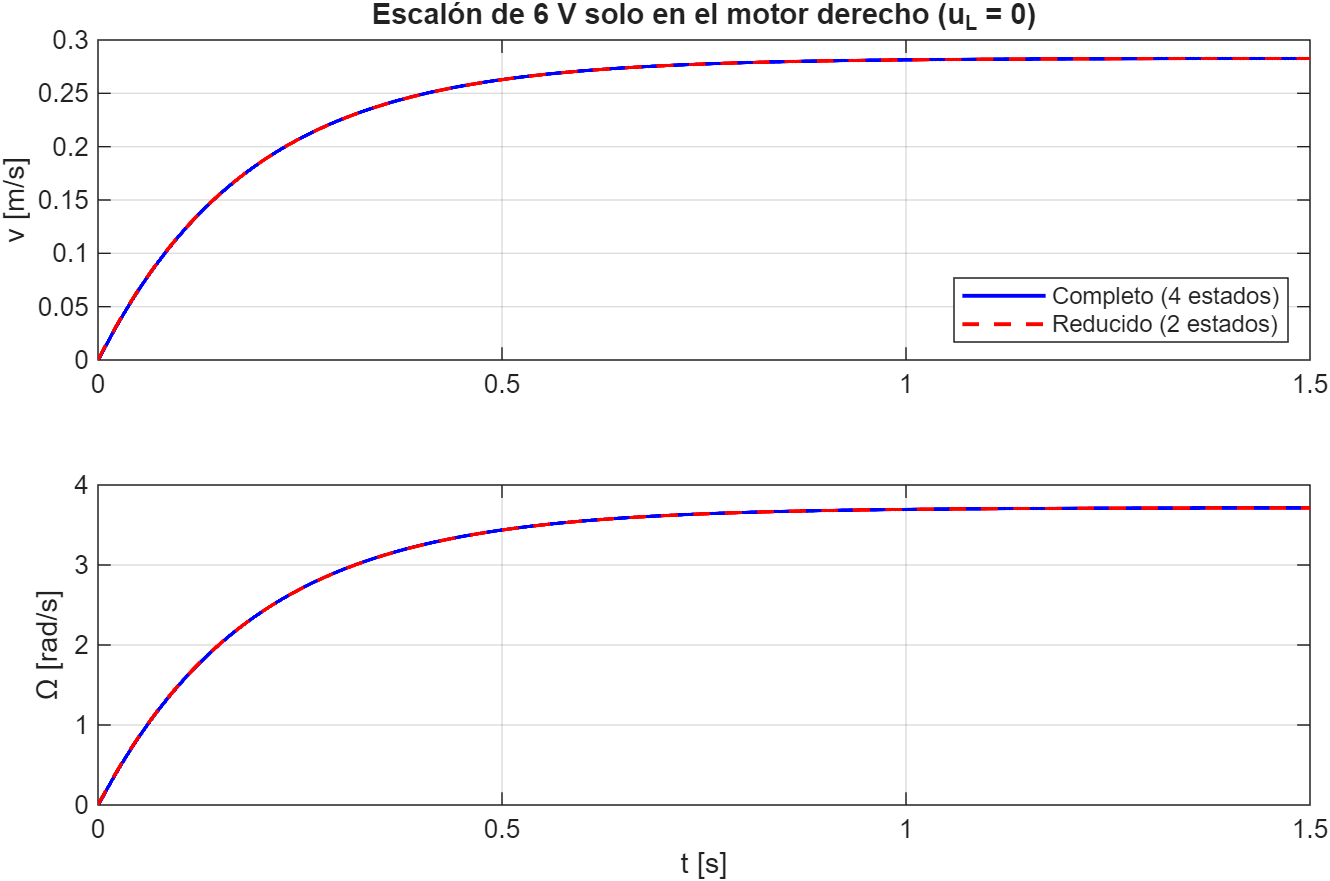
\includegraphics[width=0.78\textwidth]{p3_fig1_modelos.png}
\caption{Modelo completo (4 estados) frente al reducido (2 estados): escalón de 6~V solo en el motor derecho. El carro avanza y gira al mismo tiempo.}
\label{fig:modelos}
\end{figure}

\subsection{Matriz de transferencia y acoplamiento}
La matriz de transferencia del modelo reducido es
\begin{equation}
  G(s) = \begin{bmatrix} V(s)/U_L(s) & V(s)/U_R(s) \\ \Omega(s)/U_L(s) & \Omega(s)/U_R(s) \end{bmatrix}
  = \begin{bmatrix} \dfrac{0.2497}{s+5.298} & \dfrac{0.2497}{s+5.298} \\[10pt] \dfrac{-3.2056}{s+5.176} & \dfrac{3.2056}{s+5.176} \end{bmatrix},
  \qquad
  G(0) = \begin{bmatrix} 0.0471 & 0.0471 \\ -0.6193 & 0.6193 \end{bmatrix}.
\end{equation}
Ningún elemento de $G(s)$ es cero: \textbf{cada voltaje afecta a las dos salidas}. Subir 1~V en el motor derecho aumenta la velocidad en 0.047~m/s y el giro en 0.62~rad/s; subirlo en el izquierdo aumenta la velocidad lo mismo pero gira en sentido contrario.

En el modelo nominal, con motores idénticos, el acoplamiento está todo en la matriz $B$; la matriz $A$ es diagonal. En el carro real los motores nunca son idénticos y aparecen términos que acoplan también la dinámica. Esto se incluye en la planta de simulación para probar la robustez del controlador.

\subsection{Controlabilidad y observabilidad}
\begin{itemize}
  \item $\operatorname{rango}\big(\operatorname{ctrb}(A,B)\big) = 2$: el sistema es \textbf{controlable} con los dos voltajes. De hecho, $B$ es invertible ($\det B = 1.60 \neq 0$), así que cualquier combinación de aceleraciones de avance y de giro se puede producir.
  \item Con las medidas disponibles $y_m = [\,\omega_L\;\;\omega_R\;\;\Omega_{giro}\,]^T = C_m x$, con $C_m = \begin{bmatrix} T \\ 0\;\;1\end{bmatrix}$, se tiene $\operatorname{rango}\big(\operatorname{obsv}(A,C_m)\big)=2$: el sistema es \textbf{observable}. Hay tres medidas para dos estados, una redundancia que el filtro de Kalman aprovecha para reducir el ruido.
\end{itemize}

% ======================================================================
\section{Especificaciones de diseño}
% ======================================================================
\begin{table}[H]
\centering
\caption{Especificaciones de desempeño.}
\label{tab:especificaciones}
\begin{tabular}{p{5.6cm} c p{6.4cm}}
\toprule
Especificación & Valor & Justificación \\
\midrule
Tiempo de establecimiento de $v$ (2\%) & $\le 1.0$ s & Arranque ágil (el lazo abierto tarda 0.75 s y no tiene error nulo) \\
Sobrepaso de $v$ & $\le 5$\% & Evitar tirones \\
Tiempo de establecimiento de $\Omega$ (5\%) & $\le 1.0$ s & Giros precisos \\
Sobrepaso de $\Omega$ & $\le 10$\% & Evitar que el carro se pase en el giro \\
Error en estado estacionario & 0 & En $v$ y $\Omega$, con pendientes y frenos \\
Voltajes & $|u_L|,|u_R| \le 12$ V & Límite del driver \\
\bottomrule
\end{tabular}
\end{table}
Para $\Omega$ se usa la banda del 5\% porque el ruido del giroscopio deja una ondulación de unos $\pm0.02$~rad/s (2\% de 1~rad/s) en el valor real: con la banda del 2\% el tiempo de establecimiento medido dependería del ruido y no de la dinámica.

% ======================================================================
\section{Diseño del controlador LQR discreto MIMO}
% ======================================================================
\subsection{Discretización}
El controlador se implementará en un microcontrolador, así que se diseña directamente en tiempo discreto. Se elige $T_s = 10$~ms porque es unas 20 veces menor que la constante de tiempo mecánica ($1/5.3 \approx 0.19$~s), lo que da margen para que el lazo cerrado sea varias veces más rápido que el lazo abierto, y porque en 10~ms el encoder alcanza a contar varios pulsos a velocidades normales. El modelo \eqref{eq:reducido} se discretiza con retenedor de orden cero (\texttt{c2d}, método ZOH):
\begin{equation}
  x[k+1] = A_d\, x[k] + B_d\, u[k] + E_d\, d[k],\qquad A_d = e^{AT_s},\quad B_d = \int_0^{T_s} e^{A\tau}d\tau\, B .
\end{equation}

\subsection{Acción integral}
Para lograr error nulo en $v$ y $\Omega$ ante perturbaciones constantes se agrega un integrador discreto por cada salida:
\begin{equation}
  z[k+1] = z[k] + T_s\big(r[k] - y[k]\big), \qquad z = [\,z_v\;\; z_\Omega\,]^T,\quad r = [\,v^*\;\;\Omega^*\,]^T .
\end{equation}
El sistema aumentado, con $x_a = [\,v\;\;\Omega\;\;z_v\;\;z_\Omega\,]^T \in \R^4$, es
\begin{equation}
  x_a[k+1] = \underbrace{\begin{bmatrix} A_d & 0 \\ -T_s I_2 & I_2 \end{bmatrix}}_{A_a} x_a[k] + \underbrace{\begin{bmatrix} B_d \\ 0 \end{bmatrix}}_{B_a} u[k] + \begin{bmatrix} 0 \\ T_s I_2 \end{bmatrix} r[k],
\end{equation}
y $\operatorname{rango}\big(\operatorname{ctrb}(A_a,B_a)\big) = 4$.

\subsection{LQR discreto}
La ley de control es una sola realimentación matricial:
\begin{equation}
  \boxed{\;u[k] = \begin{bmatrix} u_L \\ u_R \end{bmatrix} = -K\,x_a[k] = -K_x \begin{bmatrix} \hat v \\ \hat\Omega \end{bmatrix} - K_z \begin{bmatrix} z_v \\ z_\Omega \end{bmatrix},\qquad K \in \R^{2\times4}\;}
\end{equation}
donde $K$ minimiza
\begin{equation}
  J = \sum_{k=0}^{\infty} \Big( x_a[k]^T Q\, x_a[k] + u[k]^T R\, u[k] \Big),
\end{equation}
y se obtiene de la ecuación algebraica de Riccati discreta (\texttt{dlqr}):
\begin{equation}
  P = A_a^TPA_a - A_a^TPB_a\big(R + B_a^TPB_a\big)^{-1}B_a^TPA_a + Q, \qquad K = \big(R + B_a^TPB_a\big)^{-1}B_a^TPA_a .
\end{equation}
En el caso MIMO el LQR es especialmente conveniente: con la ubicación de polos, en un sistema de dos entradas hay infinitas matrices $K$ que dan los mismos polos, mientras que el LQR entrega una única $K$ óptima a partir de pesos con significado físico.

\subsection{Selección de pesos}
\begin{equation}
  Q = \operatorname{diag}(q_v,\, q_\Omega,\, q_{z_v},\, q_{z_\Omega}) = \operatorname{diag}(20,\; 20,\; 600,\; 1000), \qquad R = 0.01\, I_2 .
\end{equation}
\begin{itemize}
  \item Los pesos de los integradores son los más grandes porque determinan qué tan rápido se elimina el error de seguimiento.
  \item $q_{z_\Omega} > q_{z_v}$ para que el giro responda más rápido que la velocidad: corregir el rumbo es más urgente que corregir la velocidad.
  \item Se probaron primero pesos pequeños en $\Omega$ ($Q=\operatorname{diag}(10,1,200,20)$): la velocidad cumplía, pero $\Omega$ tardaba más de 1.6~s en establecerse. Al subir $q_\Omega$ y $q_{z_\Omega}$ el giro se aceleró sin aumentar el voltaje máximo más allá de 8.2~V.
  \item $R = 0.01\,I_2$: los dos motores pesan igual porque son del mismo tipo.
\end{itemize}

\subsection{Resultado}
\begin{lstlisting}
Q  = diag([20 20 600 1000]);  Rl = 0.01*eye(2);
[K,~,pz] = dlqr(Aa, Ba, Q, Rl);
\end{lstlisting}
\begin{equation}
  K = \left[\begin{array}{cc|cc}
    30.28 & -13.60 & -159.96 & 90.88 \\
    30.28 &  13.60 & -159.96 & -90.88
  \end{array}\right].
\end{equation}
La estructura de $K$ tiene interpretación física directa:
\begin{itemize}
  \item La \textbf{primera y tercera columnas son iguales en ambas filas}: un error de velocidad hace que los dos motores suban su voltaje por igual, lo que acelera el carro sin hacerlo girar.
  \item La \textbf{segunda y cuarta columnas tienen signos opuestos}: un error de giro sube el voltaje de un motor y baja el del otro, lo que hace girar el carro sin cambiar su velocidad.
\end{itemize}
Es decir, el LQR ``descubrió'' por sí solo la descomposición en modo común (avance) y modo diferencial (giro), y reparte cada corrección entre los dos motores. Esto es lo que no hacen dos PI independientes, que solo miran el error de su propia rueda.

Los polos de lazo cerrado son
\begin{equation}
  z = \{0.9465,\; 0.9317,\; 0.8546,\; 0.1683\}\;\;\Rightarrow\;\; s = \frac{\ln z}{T_s} = \{-5.50,\; -7.07,\; -15.71,\; -178.2\}.
\end{equation}
Todos están dentro del círculo unitario. La Figura~\ref{fig:polos} muestra los polos continuos equivalentes junto a los de lazo abierto.

\begin{figure}[H]
\centering
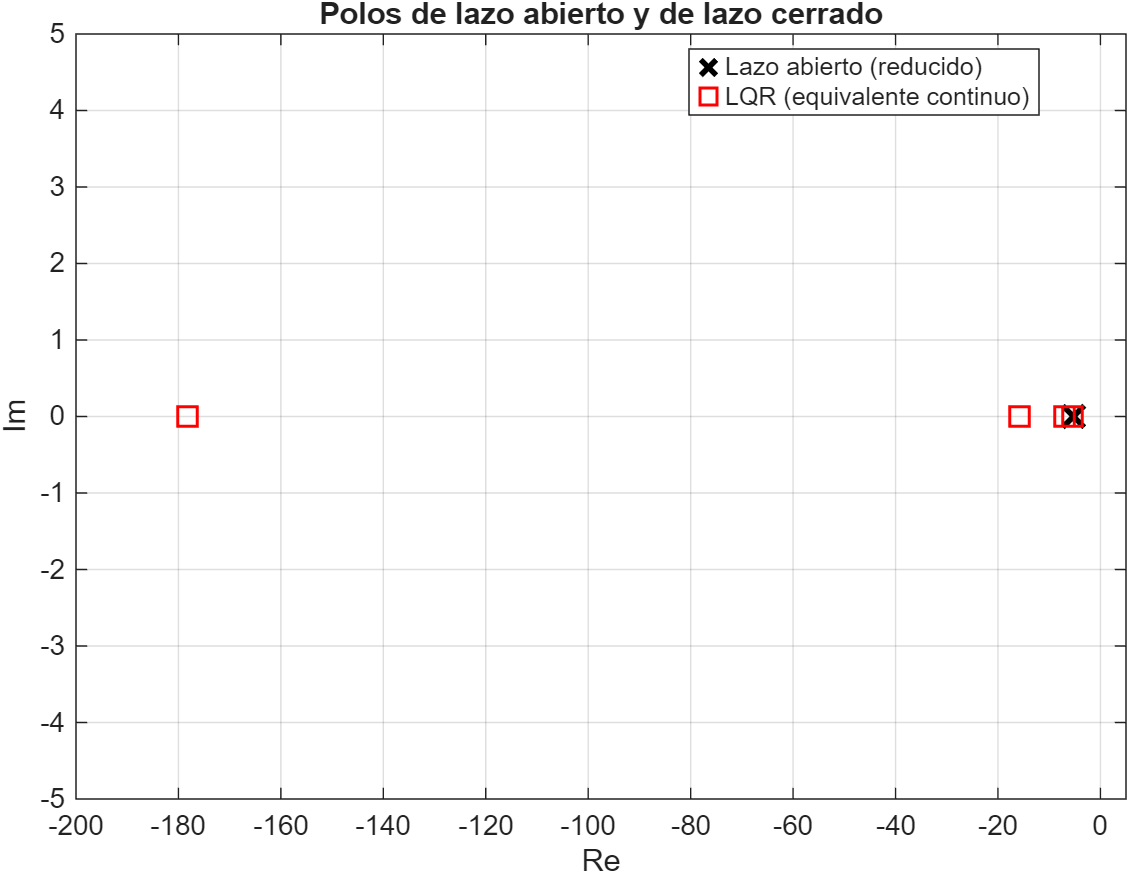
\includegraphics[width=0.66\textwidth]{p3_fig2_polos.png}
\caption{Polos de lazo abierto del modelo reducido ($\times$) y polos continuos equivalentes del lazo cerrado con LQR ($\square$).}
\label{fig:polos}
\end{figure}

La Figura~\ref{fig:escalones} muestra la matriz de respuestas al escalón del lazo cerrado nominal. Los elementos de la diagonal son las respuestas de $v$ a $v^*$ y de $\Omega$ a $\Omega^*$, sin sobrepaso y con tiempos de establecimiento (2\%) de 0.79~s y 0.56~s. Los elementos fuera de la diagonal son nulos: \textbf{el controlador desacopla el sistema}. Pedir un giro no cambia la velocidad y pedir velocidad no hace girar el carro, aunque cada voltaje afecte a ambas salidas.

\begin{figure}[H]
\centering
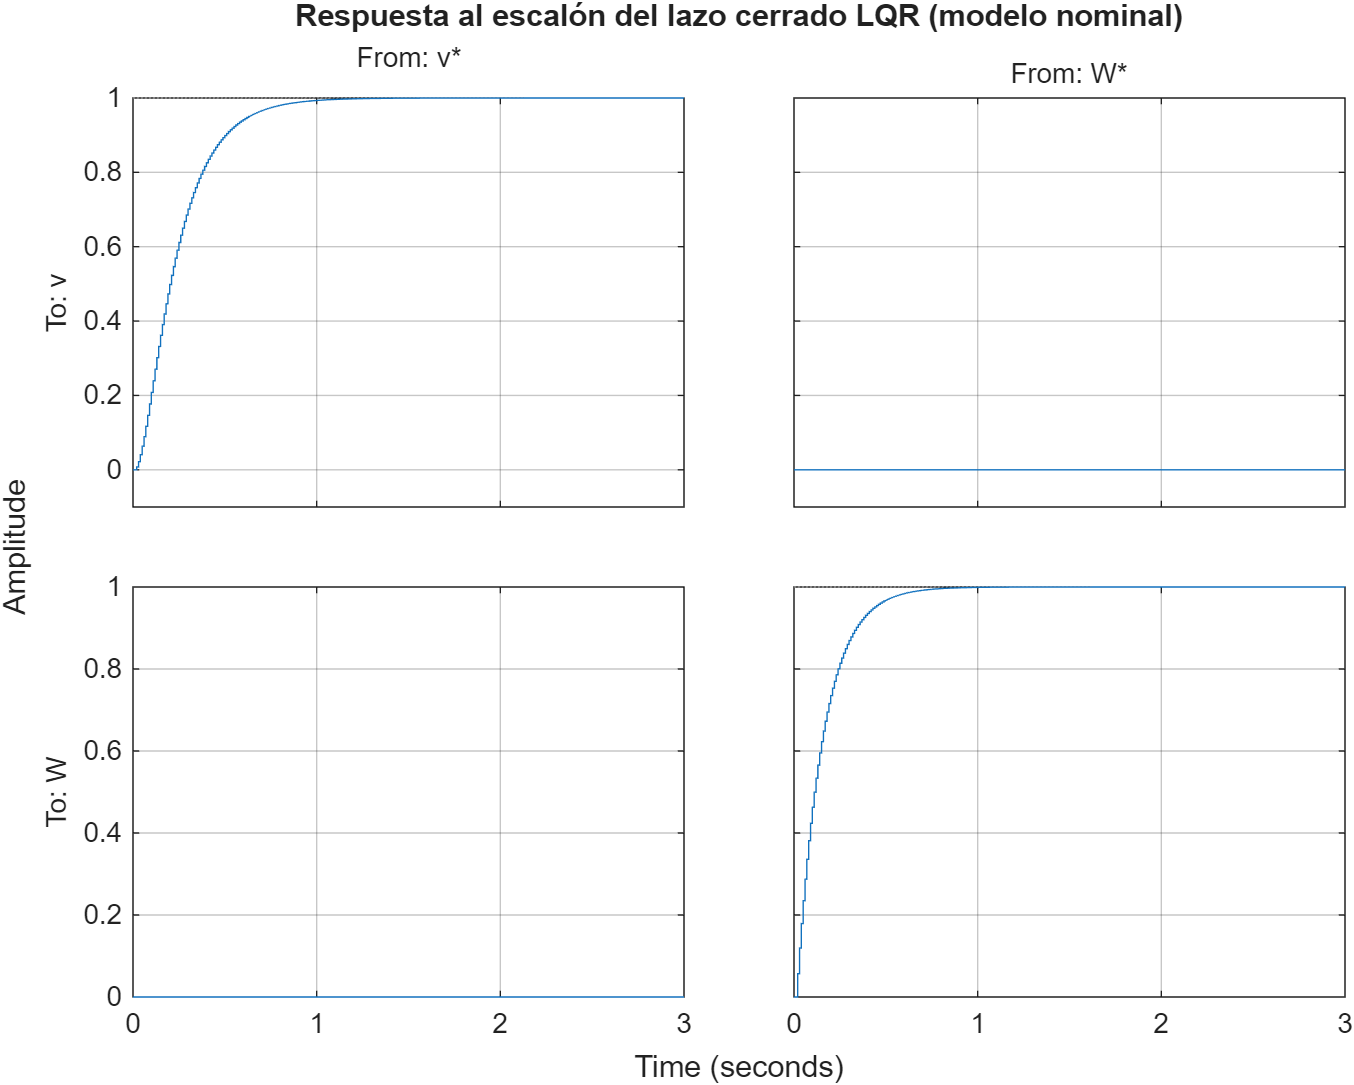
\includegraphics[width=0.74\textwidth]{p3_fig3_escalones_mimo.png}
\caption{Matriz de respuestas al escalón del lazo cerrado LQR con el modelo nominal. Fila: salida; columna: referencia.}
\label{fig:escalones}
\end{figure}

% ======================================================================
\section{Filtro de Kalman discreto con estimación de perturbaciones}
% ======================================================================
\subsection{Necesidad del estimador}
El controlador necesita $v$ y $\Omega$, pero ninguna se mide limpia:
\begin{itemize}
  \item Los encoders dan la velocidad de cada rueda contando pulsos en 10~ms. Con 1320 cuentas por vuelta, un pulso equivale a $2\pi/(1320\cdot0.01) = 0.476$~rad/s de velocidad de rueda: la medida es muy ``escalonada'' (cuantización).
  \item El giroscopio mide $\Omega$ con ruido ($\sigma = 0.02$~rad/s).
\end{itemize}
El filtro de Kalman combina las tres medidas pesándolas según su confiabilidad y usa el modelo para filtrar el ruido.

\subsection{Modelo del estimador}
Como en el punto~2, se agregan estados de perturbación para que el estimador no quede sesgado cuando aparece una pendiente o un freno. Se modelan como aceleraciones desconocidas $a_v$, $a_\Omega$ que cambian lentamente (caminata aleatoria):
\begin{equation}
  x_e = \begin{bmatrix} v \\ \Omega \\ a_v \\ a_\Omega \end{bmatrix},\qquad
  \dot x_e = \underbrace{\begin{bmatrix} A & I_2 \\ 0 & 0 \end{bmatrix}}_{A_e} x_e + \begin{bmatrix} B \\ 0 \end{bmatrix} u + w,\qquad
  y_m = \begin{bmatrix} \omega_L \\ \omega_R \\ \Omega_{giro} \end{bmatrix} = \underbrace{\begin{bmatrix} C_m & 0 \end{bmatrix}}_{C_e} x_e + \nu .
\end{equation}
Se discretiza con ZOH y se verifica que $\operatorname{rango}\big(\operatorname{obsv}(A_{de},C_e)\big) = 4$: las perturbaciones también son observables.

\subsection{Covarianzas}
\begin{itemize}
  \item \textbf{Ruido de medida $R_k$}: el error de cuantización de la velocidad por diferencia de cuentas es la resta de dos errores uniformes de ancho $q$, con varianza $q^2/6$; se usa $q^2/3$ (el doble) como valor conservador, con $q = 0.476$~rad/s. Para el giroscopio, $\sigma_g^2 = 0.02^2$. Entonces $R_k = \operatorname{diag}(q^2/3,\; q^2/3,\; 0.0004)$.
  \item \textbf{Ruido de proceso $Q_k$}: $Q_k = \operatorname{diag}(10^{-5},\,10^{-5},\,0.05,\,0.05)$. Los valores pequeños en $v$ y $\Omega$ indican confianza en el modelo; los valores mayores en $a_v$ y $a_\Omega$ permiten que las perturbaciones estimadas cambien con rapidez cuando aparece una pendiente o un freno.
\end{itemize}
La ganancia se calcula con \texttt{dlqe} en la forma de \emph{estimador actual}, que usa la medida del instante $k$ para estimar el estado del mismo instante:
\begin{equation}
  \hat x_e[k] = \hat x_e^-[k] + M\big(y_m[k] - C_e\,\hat x_e^-[k]\big),\qquad
  \hat x_e^-[k+1] = A_{de}\,\hat x_e[k] + B_{de}\,u[k].
\end{equation}
\begin{lstlisting}
[Mk,Pk] = dlqe(Ade, eye(4), Ce, Qk, Rk);
\end{lstlisting}
\begin{equation}
  M = \begin{bmatrix}
     0.0099 & 0.0099 & 0 \\
    -0.0043 & 0.0043 & 0.3492 \\
     0.3600 & 0.3600 & 0 \\
    -0.1056 & 0.1056 & 8.6417
  \end{bmatrix}.
\end{equation}
La estructura de $M$ confirma lo esperado: la velocidad $v$ se corrige con el promedio de los dos encoders (primera fila), mientras que $\Omega$ se corrige sobre todo con el giroscopio (ganancia 0.349) y casi nada con la diferencia de encoders (0.004), que es muy ruidosa por la cuantización. Los polos del estimador tienen magnitudes $|z| = \{0.609,\;0.609,\;0.774,\;0.774\}$: es más rápido que el controlador, cuyo polo dominante está en $z=0.946$.

% ======================================================================
\section{Controlador de comparación: dos PI independientes}
% ======================================================================
Para medir el beneficio del enfoque MIMO se diseñó el esquema descentralizado más común. Las referencias de las ruedas se calculan con la cinemática, $[\omega_L^*\;\omega_R^*]^T = T\,[v^*\;\Omega^*]^T$, y cada motor tiene su propio PI discreto:
\begin{equation}
  u_j[k] = K_p\, e_j[k] + K_i\, T_s \sum_{n=0}^{k} e_j[n], \qquad e_j = \omega_j^* - \hat\omega_j,\qquad K_p = 0.3~\tfrac{\text{V$\cdot$s}}{\text{rad}},\; K_i = 3~\tfrac{\text{V}}{\text{rad}}.
\end{equation}
Para que la comparación sea justa, el PI usa las mismas velocidades estimadas por el filtro de Kalman ($\hat\omega = T\hat x$). Las ganancias se ajustaron para obtener un tiempo de establecimiento similar al del LQR: con ganancias mayores el sobrepaso subía por encima del 10\% y el voltaje llegaba a la saturación.

% ======================================================================
\section{Implementación en simulación}
\label{sec:implementacion}
% ======================================================================
El controlador se implementa en una simulación que reproduce lo que pasaría en el carro real. A diferencia del modelo de diseño, la planta simulada incluye:
\begin{enumerate}
  \item \textbf{Modelo completo con corrientes}: se integran las cuatro ecuaciones (velocidades y corrientes) con el método de Euler y paso $\Delta t = 0.1$~ms, más de seis veces menor que $\tau_e$.
  \item \textbf{Motores desiguales}: el motor derecho tiene $K_t$ y $K_e$ un 8\% menores y $R$ un 5\% mayor que el izquierdo, como podría pasar por tolerancias de fabricación. El controlador se diseñó con motores idénticos.
  \item \textbf{Fricción de Coulomb}: resistencia a la rodadura $0.02\,mg\,\operatorname{sign}(v)$ y fricción seca en cada reductora de 0.01~N$\cdot$m. Para evitar discontinuidades numéricas el signo se aproxima con una tangente hiperbólica.
  \item \textbf{Saturación} de los voltajes en $\pm12$~V.
  \item \textbf{Encoders cuantizados}: se acumula el ángulo real de cada rueda, se convierte a cuentas enteras y la velocidad se calcula por diferencia de cuentas en cada $T_s$.
  \item \textbf{Giroscopio con ruido} gaussiano de $\sigma = 0.02$~rad/s.
  \item \textbf{Perturbaciones}: una pendiente de 10° (fuerza de $-mg\sin 10^\circ = -2.55$~N) y un freno de 0.15~N$\cdot$m sobre la rueda derecha, por ejemplo porque pisa pasto o arena.
  \item \textbf{Posición del carro}: se integran $\dot X = v\cos\psi$, $\dot Y = v\sin\psi$, $\dot\psi=\Omega$ para dibujar la trayectoria.
\end{enumerate}

El controlador corre cada 10~ms, igual que en el microcontrolador. El ciclo de control (función \texttt{simular\_carro} del script) es:
\begin{lstlisting}
cnt   = floor(th/qth);                     % cuentas de los encoders
wmeas = (cnt - cntp)*qth/Ts;  cntp = cnt;  % velocidad de cada rueda
Wg    = x(2) + sig_g*randn;                % giroscopio
xe    = xe + Mk*([wmeas; Wg] - Ce*xe);     % correccion de Kalman
u     = -K(:,1:2)*xe(1:2) - K(:,3:4)*z;    % ley de control MIMO
z     = z + Ts*(ref - xe(1:2));            % integradores
u     = min(max(u,-12),12);                % saturacion
xe    = Ade*xe + Bde*u;                    % prediccion de Kalman
% ... la planta no lineal avanza 100 pasos de 0.1 ms con u constante
\end{lstlisting}

Se hicieron tres pruebas:
\begin{itemize}
  \item \textbf{Prueba A}: escalón de velocidad $v^* = 0.5$~m/s con $\Omega^* = 0$ (arrancar en línea recta).
  \item \textbf{Prueba B}: escalón de giro $\Omega^* = 1$~rad/s con el carro avanzando a 0.5~m/s.
  \item \textbf{Prueba C}: recorrido completo de 11~s: arranque a 0.5~m/s en $t=0.5$~s, giro de 1~rad/s entre $t=3$ y $t=5$~s (debe girar 2~rad, unos 115°), pendiente de 10° desde $t=6.5$~s y freno en la rueda derecha desde $t=8.5$~s.
\end{itemize}

% ======================================================================
\section{Resultados}
% ======================================================================
\subsection{Prueba A: arranque en línea recta}
\begin{figure}[H]
\centering
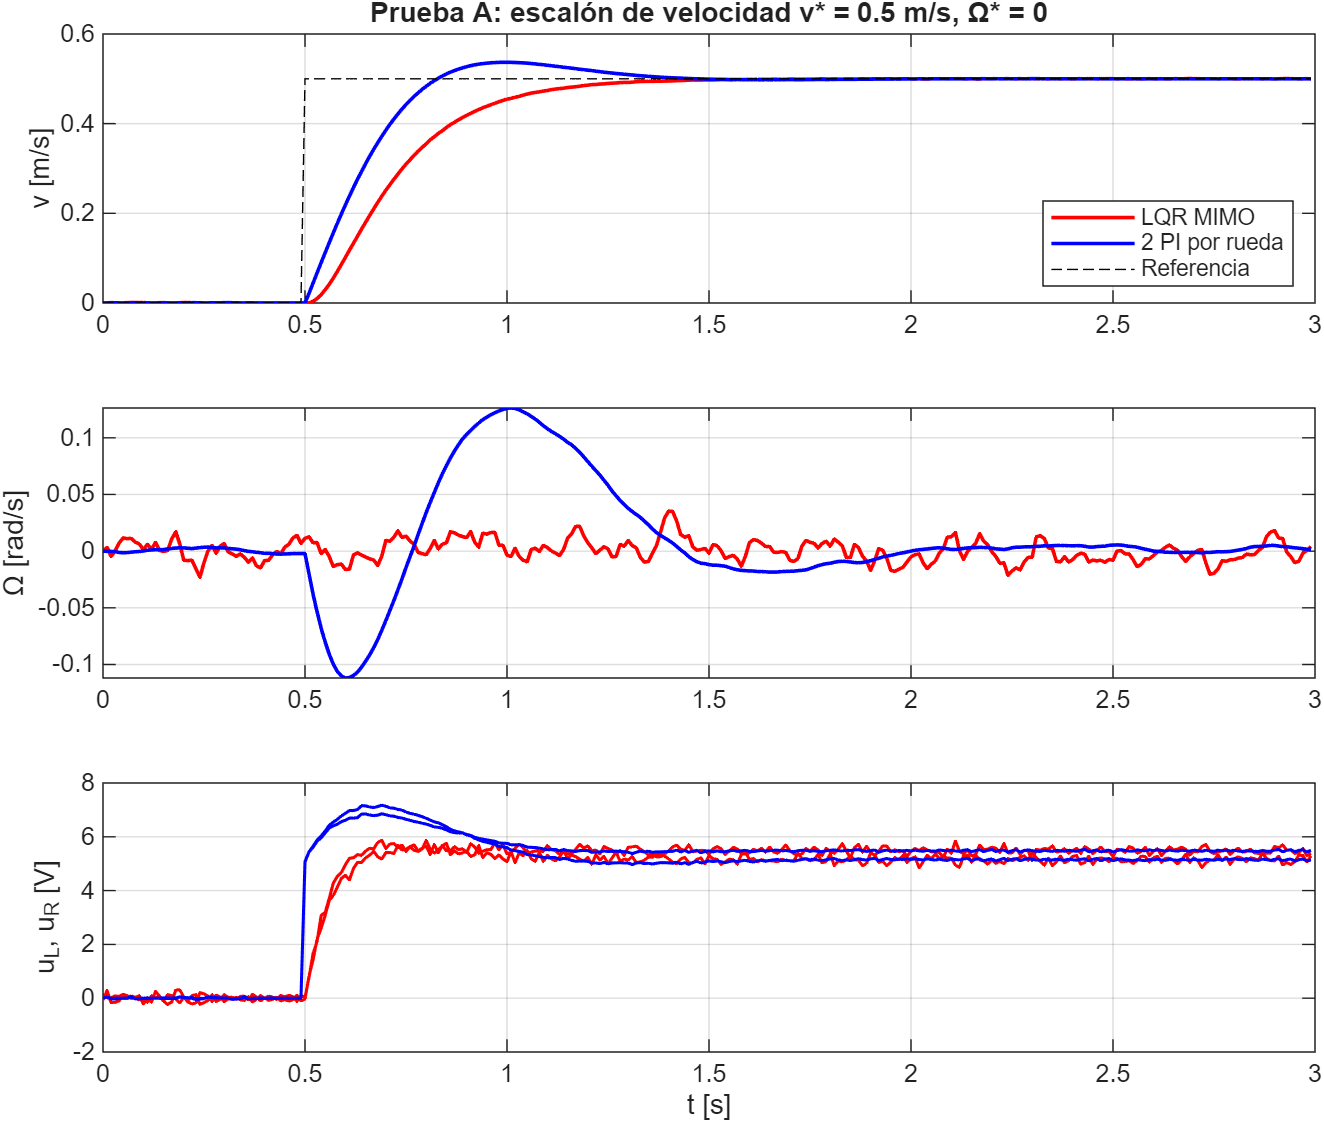
\includegraphics[width=0.76\textwidth]{p3_fig4_prueba_A.png}
\caption{Prueba A: escalón de velocidad. Arriba, velocidad; centro, velocidad de giro (debería ser cero); abajo, voltajes de ambos motores.}
\label{fig:pruebaA}
\end{figure}
La Figura~\ref{fig:pruebaA} muestra la diferencia principal entre los dos controladores. Al arrancar, el motor derecho es más débil que el izquierdo. Con los dos PI cada rueda corrige su propio error de forma independiente; durante el transitorio el motor izquierdo va adelante y el carro gira primero a la derecha y luego a la izquierda, con un pico de $|\Omega| = 0.126$~rad/s. El LQR MIMO ve el error de giro como un estado más y lo corrige en cuanto aparece, repartiendo el voltaje entre los dos motores: el giro inducido se queda en 0.035~rad/s, del orden del ruido del giroscopio. Además, el PI tiene un sobrepaso de 7.4\% en velocidad (fuera de especificación), mientras que el LQR no tiene sobrepaso.

\subsection{Prueba B: giro a velocidad constante}
\begin{figure}[H]
\centering
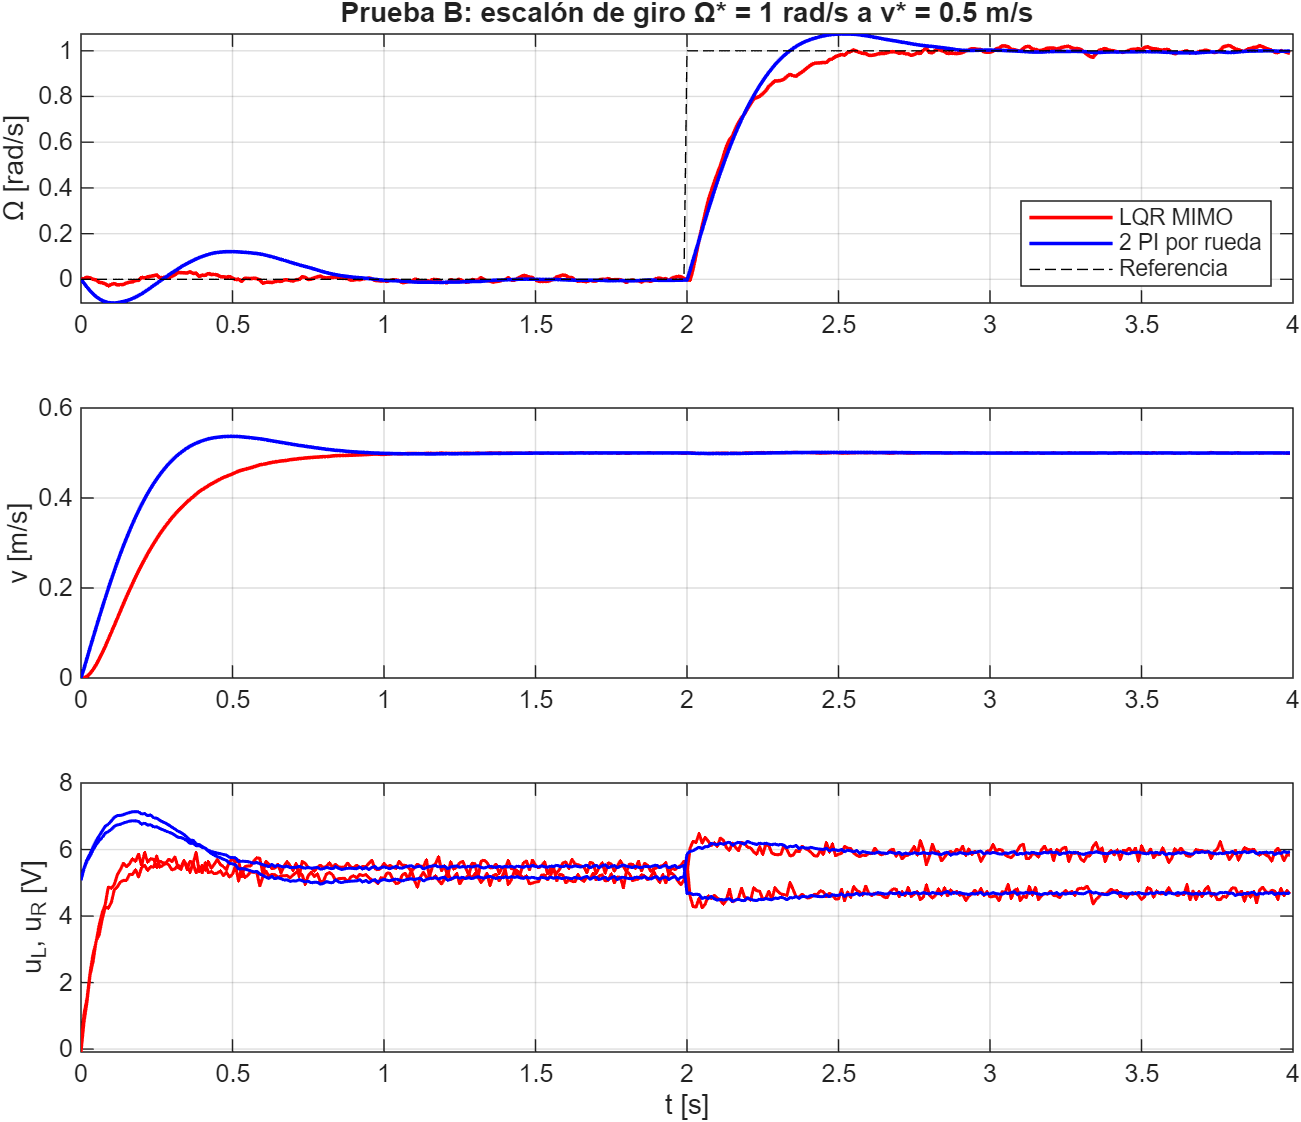
\includegraphics[width=0.76\textwidth]{p3_fig5_prueba_B.png}
\caption{Prueba B: escalón de giro de 1~rad/s a 0.5~m/s. Arriba, velocidad de giro; centro, velocidad de avance; abajo, voltajes.}
\label{fig:pruebaB}
\end{figure}
En la Figura~\ref{fig:pruebaB} el LQR alcanza el giro deseado en 0.46~s con 2.4\% de sobrepaso; los PI tardan 0.65~s y se pasan un 7.3\%. En ambos casos la velocidad de avance prácticamente no cambia durante el giro (desviación de 1.2 a 1.4~mm/s), porque el giro solo exige una diferencia de voltajes que se reparte simétricamente.

\subsection{Prueba C: recorrido completo con perturbaciones}
\begin{figure}[H]
\centering
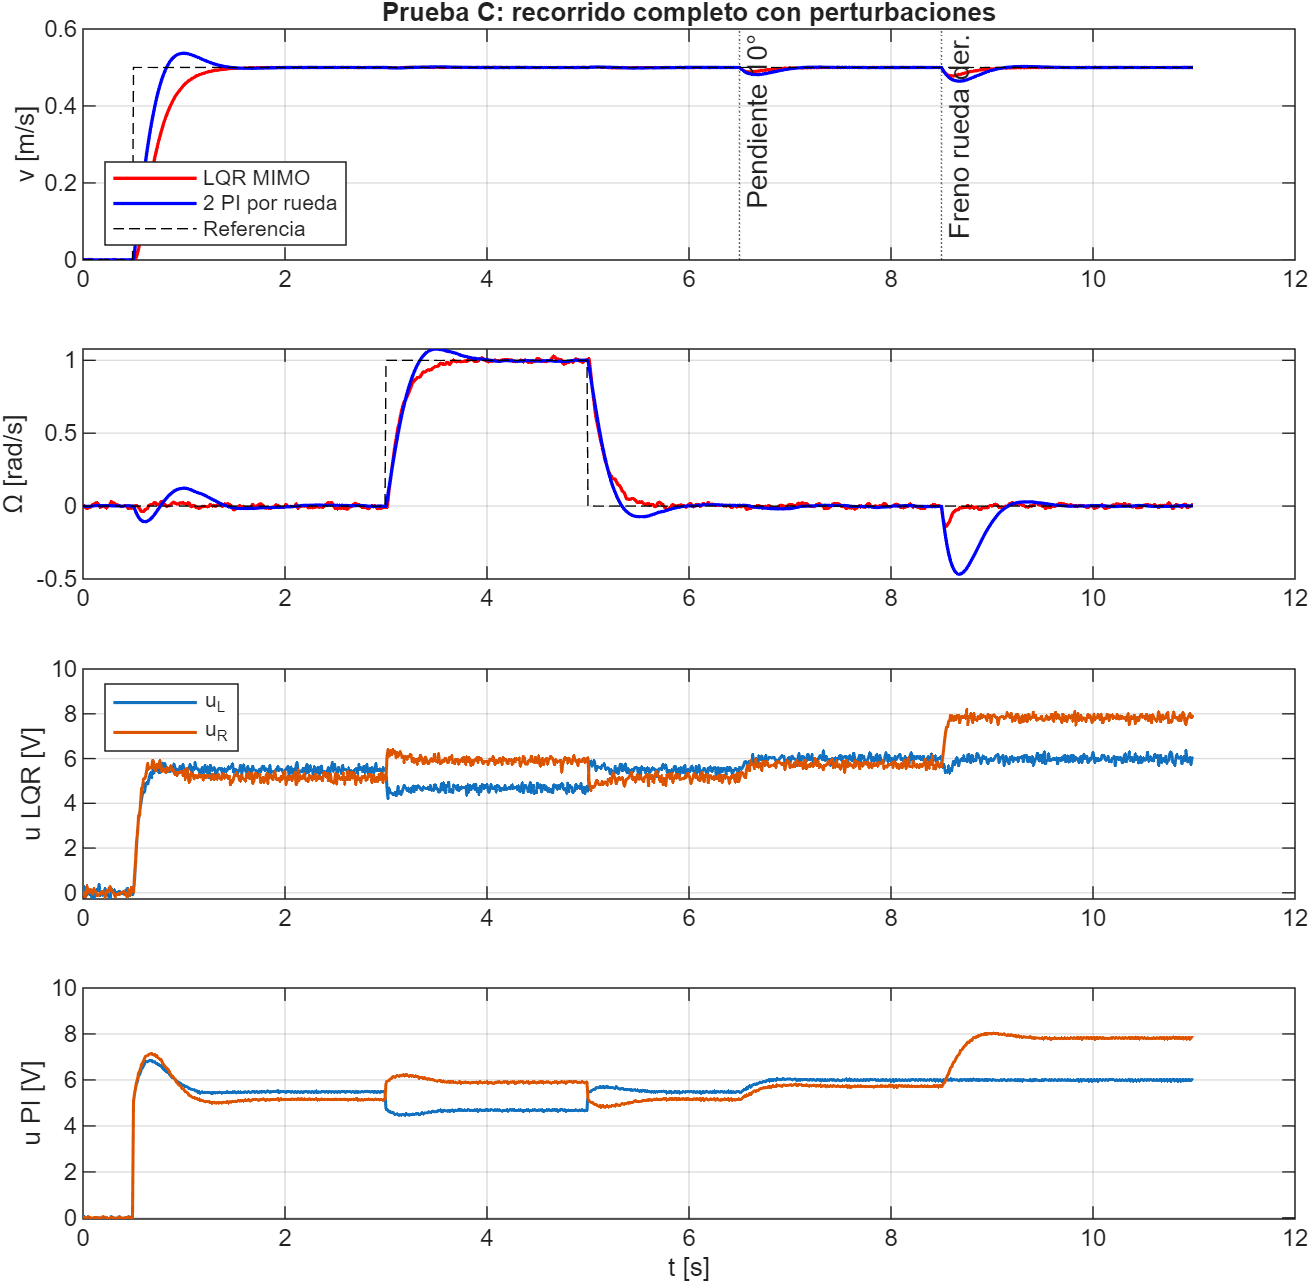
\includegraphics[width=0.80\textwidth]{p3_fig6_prueba_C.png}
\caption{Prueba C: velocidad, velocidad de giro y voltajes del LQR y de los PI durante el recorrido completo.}
\label{fig:pruebaC}
\end{figure}
En la Figura~\ref{fig:pruebaC} se observan los efectos de las perturbaciones:
\begin{itemize}
  \item \textbf{Pendiente} ($t=6.5$~s): ambos controladores suben el voltaje de los dos motores por igual y la velocidad cae menos de 2~cm/s antes de recuperarse. El LQR se desvía 0.012~m/s y el PI 0.018~m/s.
  \item \textbf{Freno en la rueda derecha} ($t=8.5$~s): la diferencia es clara. El freno frena la rueda derecha y el carro tiende a girar a la derecha. Con los PI, solo la rueda derecha reacciona y el carro llega a girar a $-0.47$~rad/s antes de corregirse. El LQR interpreta el freno como un error de giro y ajusta ambos motores, limitando el giro a $-0.14$~rad/s, tres veces menos.
  \item En estado estacionario, ambos controladores terminan con $u_R \approx 7.8$~V y $u_L \approx 6$~V. Es el voltaje que necesita la rueda frenada, y lo encuentran los integradores sin conocer el freno.
\end{itemize}

\subsection{Filtro de Kalman}
\begin{figure}[H]
\centering
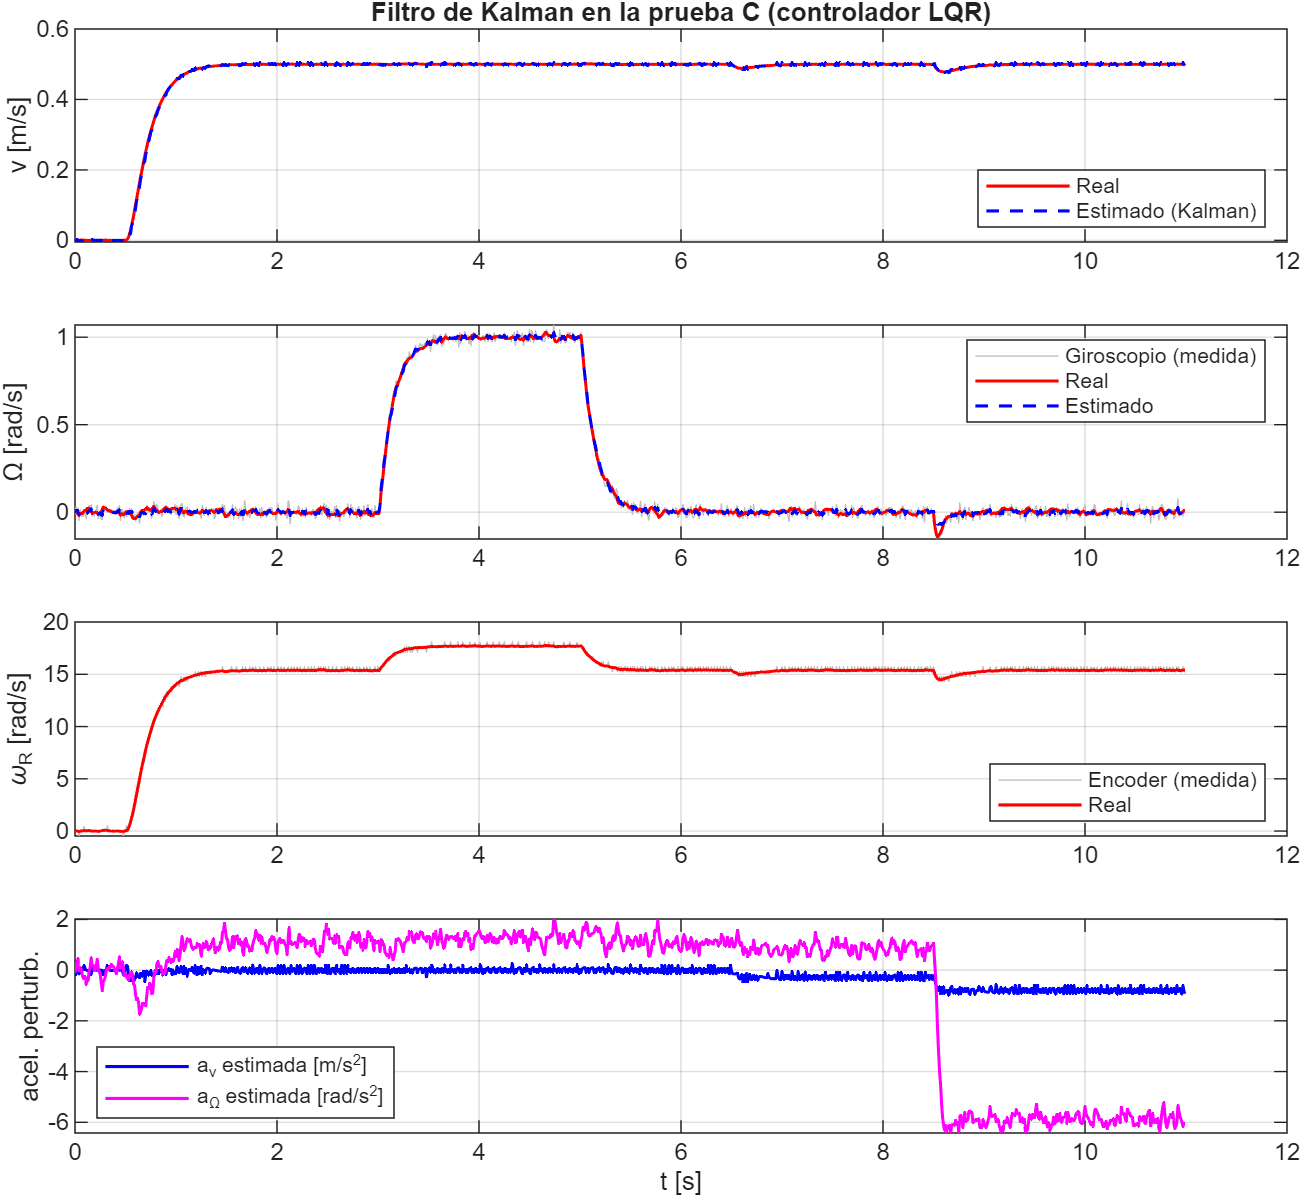
\includegraphics[width=0.80\textwidth]{p3_fig7_kalman.png}
\caption{Filtro de Kalman en la prueba C: estimación de $v$ y $\Omega$ frente a los valores reales, medida del giroscopio (gris), medida del encoder derecho (gris) y aceleraciones de perturbación estimadas.}
\label{fig:kalman}
\end{figure}
La Figura~\ref{fig:kalman} muestra que las estimaciones de $v$ y $\Omega$ siguen a los valores reales a pesar de que las medidas son ruidosas (giroscopio) o escalonadas (encoder). Las perturbaciones estimadas tienen sentido físico:
\begin{itemize}
  \item Desde $t=6.5$~s, $\hat a_v$ baja a unos $-0.25$~m/s$^2$, que es justo $-mg\sin 10^\circ/M = -2.55/10.07$.
  \item Desde $t=8.5$~s, $\hat a_\Omega$ salta a unos $-6$~rad/s$^2$. El freno de 0.15~N$\cdot$m equivale a una fuerza de $0.15/r = 4.6$~N en la rueda derecha y a un torque de giro de $4.6\cdot d/2 = 0.35$~N$\cdot$m, que dividido por $J_z$ da $5.9$~rad/s$^2$.
  \item Antes del freno, $\hat a_\Omega \approx 1$~rad/s$^2$. No es una perturbación externa: es la diferencia entre los motores real y nominal. El estimador la absorbe como una perturbación más, y por eso el controlador no queda sesgado a pesar de haberse diseñado con motores idénticos.
\end{itemize}

\subsection{Trayectoria}
\begin{figure}[H]
\centering
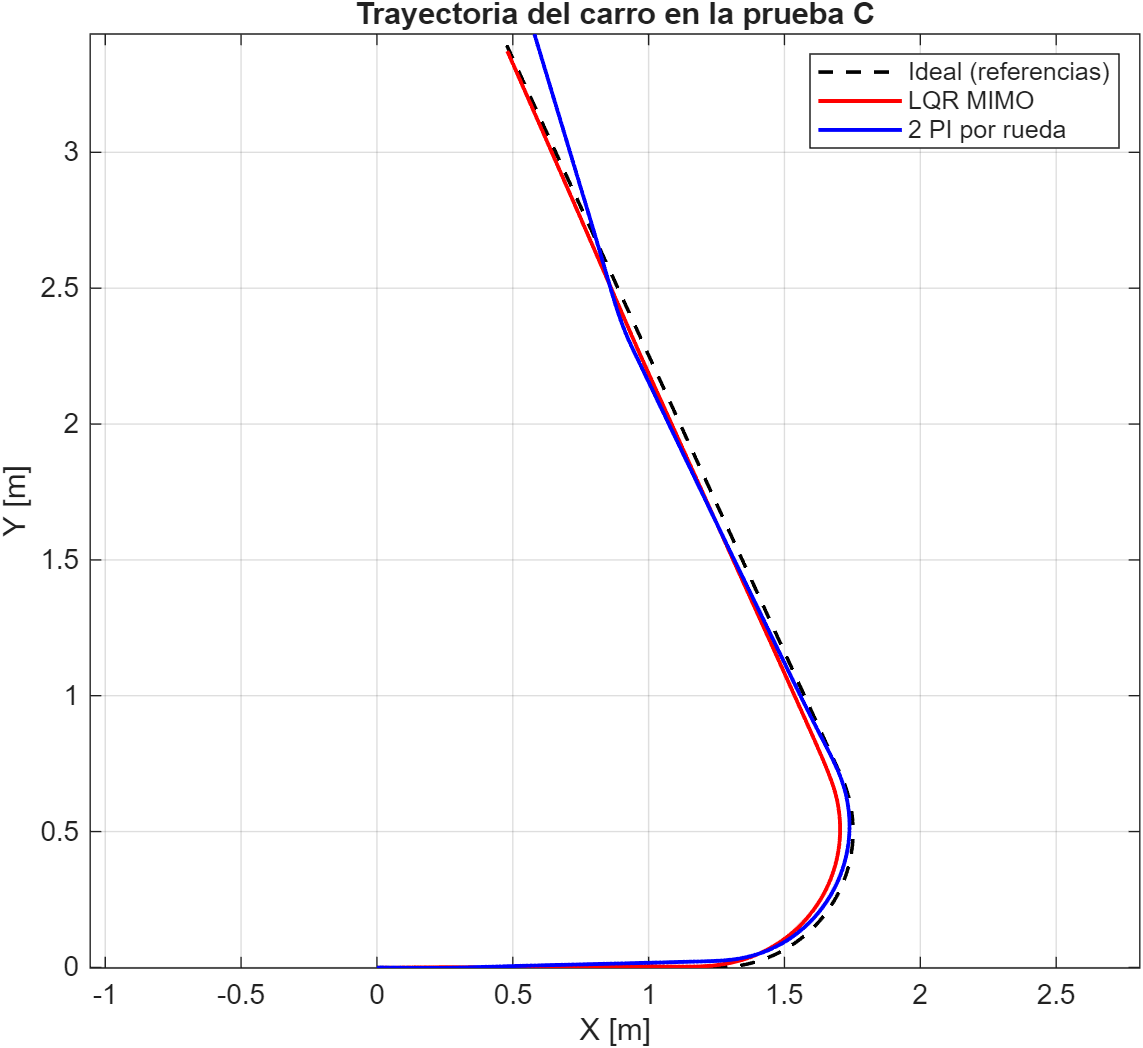
\includegraphics[width=0.62\textwidth]{p3_fig8_trayectoria.png}
\caption{Trayectoria del carro en la prueba C: ideal (calculada con las referencias), LQR MIMO y PI por rueda.}
\label{fig:trayectoria}
\end{figure}
La Figura~\ref{fig:trayectoria} resume el efecto de todo lo anterior sobre lo que realmente importa en un vehículo: por dónde va. Los dos controladores siguen la curva, pero los errores de giro de los PI se acumulan en el rumbo: al final el carro con PI apunta a 1.864~rad en vez de 2.000~rad (7.8° de error) y se va separando de la trayectoria ideal. Con el LQR el rumbo final es 1.986~rad (0.8° de error).

\subsection{Resumen de resultados}
\begin{table}[H]
\centering
\caption{Resumen de resultados de la simulación no lineal.}
\label{tab:resultados}
\begin{tabular}{l c c c}
\toprule
Parámetro & Especificación & LQR MIMO & 2 PI por rueda \\
\midrule
A: tiempo de establecimiento de $v$ (2\%) [s] & $\le 1.0$ & 0.750 & 0.790 \\
A: sobrepaso de $v$ [\%] & $\le 5$ & 0.16 & 7.37 \\
A: $|\Omega|$ máximo inducido por el arranque [rad/s] & -- & 0.035 & 0.126 \\
B: tiempo de establecimiento de $\Omega$ (5\%) [s] & $\le 1.0$ & 0.460 & 0.650 \\
B: sobrepaso de $\Omega$ [\%] & $\le 10$ & 2.35 & 7.34 \\
B: $|v-v^*|$ máximo durante el giro [m/s] & -- & 0.0012 & 0.0014 \\
C: $|v-v^*|$ máximo por la pendiente [m/s] & -- & 0.0118 & 0.0184 \\
C: $|\Omega|$ máximo por el freno en una rueda [rad/s] & -- & 0.143 & 0.467 \\
C: rumbo final $\psi$ [rad] (ideal 2.000) & -- & 1.986 & 1.864 \\
Voltaje máximo en todas las pruebas [V] & $\le 12$ & 8.19 & 8.04 \\
\bottomrule
\end{tabular}
\end{table}

% ======================================================================
\section{Análisis de resultados}
% ======================================================================
\begin{itemize}
  \item \textbf{Cumplimiento de especificaciones.} El LQR MIMO cumple todas las especificaciones de la Tabla~\ref{tab:especificaciones} sobre la planta no lineal, con motores desiguales y sensores reales, sin llegar a la saturación (8.2~V de 12~V). Los dos PI cumplen los tiempos pero no el sobrepaso de velocidad (7.4\% frente a 5\%).

  \item \textbf{Por qué gana el controlador MIMO.} Los dos PI controlan bien la velocidad de cada rueda, pero el error que importa en un carro es la \emph{diferencia} entre las ruedas, porque esa diferencia es el giro. Como cada PI ignora lo que hace el otro, cualquier diferencia entre los motores o entre las cargas de las ruedas se convierte en un giro indeseado que nadie corrige directamente. El LQR tiene a $\Omega$ y a su integral como estados, así que corrige el giro de inmediato y reparte la corrección entre los dos motores. Esto se ve en la estructura de $K$ (modo común y modo diferencial) y en los resultados: tres a cuatro veces menos giro indeseado y diez veces menos error de rumbo.

  \item \textbf{Desacoplamiento.} Con el modelo nominal, el LQR desacopla por completo las dos salidas (Figura~\ref{fig:escalones}). Con la planta real el desacoplamiento no es perfecto por la diferencia entre motores, pero los integradores y el estimador de perturbaciones compensan casi todo el efecto.

  \item \textbf{Papel del filtro de Kalman.} El estimador permite usar sensores baratos: un encoder de baja resolución (0.476~rad/s por cuenta en 10~ms) y un giroscopio ruidoso. Combinarlos da estimaciones mucho más limpias que cualquiera de los dos por separado. Los estados de perturbación, como en el punto~2, evitan que las estimaciones queden sesgadas con la pendiente o el freno, y además absorben la diferencia entre los motores.

  \item \textbf{Robustez.} El controlador se diseñó con motores idénticos, sin fricción de Coulomb y sin dinámica de corriente, y funcionó bien con todo eso presente. Esto es coherente con los márgenes de robustez del LQR y con la acción integral.

  \item \textbf{Limitaciones.}
  \begin{itemize}
    \item El modelo supone que las ruedas no deslizan. En giros rápidos o sobre superficies lisas habría que agregar un modelo de llanta.
    \item Los parámetros del carro ($m$, $c_v$, $c_\omega$) son supuestos y deberían identificarse con pruebas.
    \item No hay esquema anti-windup: si una perturbación grande saturara los motores, los integradores podrían cargarse en exceso.
    \item El ruido del giroscopio se modeló blanco y sin deriva (\emph{bias}). Un giroscopio real tiene deriva lenta; los estados de perturbación del estimador la absorberían en parte.
  \end{itemize}
\end{itemize}

% ======================================================================
\section{Conclusiones}
% ======================================================================
\begin{itemize}
  \item Se obtuvo un modelo en espacio de estados del carro de tracción trasera con dos motores independientes, combinando la cinemática de las ruedas, la dinámica del chasis y el modelo del motor del punto~2. La forma generalizada $M_b\dot x = T^TNK_t i - (\cdots)x$ muestra que la inercia de los rotores, multiplicada por $N^2$, domina la dinámica: la masa equivalente es casi siete veces la real.
  \item El sistema es MIMO y acoplado: los dos voltajes afectan a la velocidad y al giro, y ningún elemento de la matriz de transferencia es cero. Es controlable con los dos motores y observable con los encoders y el giroscopio.
  \item Como $\tau_e \ll T_s$, la dinámica eléctrica se puede eliminar del modelo de diseño. La simulación con el modelo completo confirmó que la reducción no afecta el desempeño.
  \item Un LQR discreto con acción integral sobre $v$ y $\Omega$ produce una sola matriz de ganancias $2\times4$ que descompone automáticamente cada corrección en un modo común (avance) y un modo diferencial (giro), y desacopla el sistema nominal.
  \item Un filtro de Kalman discreto con estados de perturbación combina encoders de baja resolución y un giroscopio ruidoso, estima la pendiente y el freno con valores físicamente correctos y absorbe la diferencia entre los motores.
  \item Implementado en simulación sobre una planta no lineal con motores desiguales, fricción de Coulomb, saturación, cuantización, ruido y perturbaciones, el LQR MIMO cumple todas las especificaciones. Frente a dos PI independientes, reduce el giro indeseado en el arranque de 0.126 a 0.035~rad/s, el giro causado por un freno en una rueda de 0.47 a 0.14~rad/s y el error de rumbo al final del recorrido de 7.8° a 0.8°.
  \item El trabajo cierra el ciclo del proyecto: el modelo de un motor (punto~2) se convirtió en la pieza de un sistema MIMO cuyo controlador se diseñó con LQR, la técnica que en el punto~2 resultó más conveniente.
\end{itemize}

% ======================================================================
\appendix
\section{Correspondencia con el script de MATLAB}
\label{ap:script}
% ======================================================================
El archivo \texttt{punto3\_carro\_MIMO.m} se ejecuta de una sola vez (unos 30~s). Genera las figuras con prefijo \texttt{p3\_} en la carpeta \texttt{IMAGENES/} y escribe los resultados numéricos en \texttt{resultados\_punto3.txt}. El ruido se genera con semilla fija (\texttt{rng(1)}), así que los resultados son reproducibles.

\begin{table}[H]
\centering
\caption{Secciones del script y resultados que producen.}
\begin{tabular}{c l l}
\toprule
Sección & Contenido & Resultado en este documento \\
\midrule
1 & Parámetros del motor y del carro & Tabla~\ref{tab:parametros} \\
2 & Modelo completo $A_f$, $B_f$ & Sección 5.1 \\
3 & Modelo reducido y comparación & Figura~\ref{fig:modelos} \\
4 & \texttt{ctrb}, \texttt{obsv}, \texttt{tf}, \texttt{dcgain} & Secciones 5.2 y 5.3 \\
5 & \texttt{c2d}, sistema aumentado, \texttt{dlqr} & Sección 7 \\
6 & Filtro de Kalman (\texttt{dlqe}) & Sección 8 \\
7 & PI por rueda & Sección 9 \\
8 & Escalones del lazo cerrado y polos & Figuras~\ref{fig:polos} y \ref{fig:escalones} \\
9 & Simulación no lineal (\texttt{simular\_carro}) & Figuras~\ref{fig:pruebaA}--\ref{fig:trayectoria} \\
10 & Métricas & Tabla~\ref{tab:resultados} \\
\bottomrule
\end{tabular}
\end{table}

\end{document}
